\documentclass[11pt, twocolumn]{article}
% -------------------------------------------------------------------
\usepackage{graphicx}
\usepackage{float}
% -------------------------------------------------------------------
% Title setup
\title{\renewcommand{\baselinestretch}{1.17}\bf%
\uppercase{A short investigation of the exponential function}
}
% -------------------------------------------------------------------
% Author
\author{Søren Skovgaard Balling}
% -------------------------------------------------------------------

% Initialize the document

\begin{document}

\date{March 2, 2022}

\maketitle

\section{Introduction}
The exponential function is a mathematical function denoted by $f(x)=\exp(x)$ or $e^{x}$ (where the argument $x$ is written as an exponent). It can be defined in several equivalent ways. Its ubiquitous occurrence in pure and applied mathematics led mathematician Walter Rudin to opine that the exponential function is "the most important function in mathematics". Its value at $1$, $e=\exp(1)\simeq 2.718$ is a mathematical constant called Euler's number.
\section{Numerical application}
In order to numerically compute the exponential function, a quick-and-dirty implementation has been introduced. In particular, this implementation is based on a power series representation of the exponential function, see equation (\ref{eq:power_series}) below
\begin{equation} \label{eq:power_series}
\exp(x) = \sum_{k = 0}^{\infty} \frac{x^k}{k!} \simeq 1 + x + \frac{x^2}{2} + \frac{x^3}{6} + \frac{x^4}{24} + \cdots
\end{equation}
For the purpose of this particular function, the leading 10 orders in the expansion has been included. Granted that the function recieves a negative value $-x$, the function is called recursively as $(e^{-x})^{-1}$. Also, if the function is called with a value $x$ greater than a certain precision $1/8$, the function is called recursively as $(e^{x/2})^{2}$ in order to retrieve the required precision. 
\section{Validation}
In order to validate the numerically implemented exponential function, a comparison to table values is done. The result can be seen in figure \ref{fig:validation}. The correlation is acceptable.
\begin{figure}
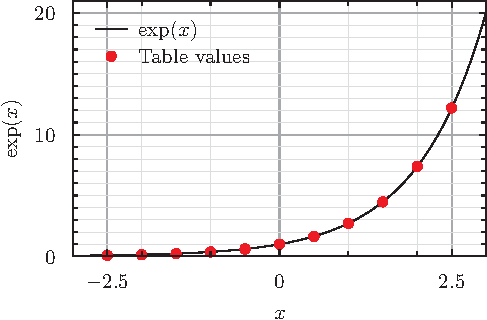
\includegraphics{exp_pyxplot.pdf}
\caption{Validation of the function with regards to tabulated values.}
\label{fig:validation}
\end{figure}

\end{document}